\documentclass[cjk,slidestop,compress,mathserif,blue]{beamer}
%dvipdfm选项是关键,否则编译统统通不过
%beamer的颜色选项定义的是导航条和标题的颜色(即关键词structure的颜色)

%%%%%%%%%%%%%%%%仅限于XeTeX可使用的宏包%%%%%%%%%%%%%%%%%%%%%%%%%%%%
\usepackage{fontspec,xunicode,xltxtra,beamerthemesplit}
%\usepackage{beamerthemesplit}
\usepackage{handoutWithNotes}		%(讲义)在打印PPT的时候会留出给每一页做注释的部分
\usepackage{xeCJK}
\setCJKmainfont[BoldFont=黑体, ItalicFont=楷体, BoldItalicFont=仿宋]{黑体}
%\setsansfont[Mapping=tex-text]{Adobe 黑体 Std}
%如果装了Adobe Acrobat,可在font.conf中配置Adobe字体的路径以使用其中文字体
%也可直接使用系统中的中文字体如SimSun,SimHei,微软雅黑 等
%原来beamer用的字体是sans family;注意Mapping的大小写,不能写错

\usepackage{listings} 
\lstset{language=Matlab}%代码语言使用的是matlab 
\lstset{breaklines}%自动将长的代码行换行排版 
\lstset{extendedchars=false}%解决代码跨页时,章节标\dots

%%%%%%%%   确定标题和导航条结构的框架     %%%%%%%%%%%%
\usepackage{beamerthemeshadow}                       %
%\usepackage{beamerthemeclassic}%导航条色与背景色一致%
%%%%%%%%%%%%%%%%%%%%%%%%%%%%%%%%%%%%%%%%%%%%%%%%%%%%%%
\setbeamerfont{roman title}{size={}}
%\usepackage{CJK} % CJK 中文支持                                  %
\usepackage{amsmath,amsthm,amsfonts,amssymb,bm}
\usepackage{bbding}
\usepackage{mathrsfs}
\usepackage{xcolor}                                        %使用默认允许使用颜色
\usepackage{hyperref} 
\usepackage{graphicx}
\usepackage{subfigure}           %图片跨页
\usepackage{animate}		 %插入动画
\usepackage{tikz}		 %绘图工具
\usepackage{caption}
\captionsetup{font=footnotesize}

%\usepackage[version=3]{mhchem}		%化学公式
\usepackage{chemformula}
\usepackage{chemfig}		%化学公式

\usepackage{multirow}
\usepackage{makecell}		%允许单元格内换行

\usepackage[dvipdfmx]{movie15_dvipdfmx} %插入视频
%\usepackage{handoutWithNotes}		%(讲义)在打印PPT的时候会留出给每一页做注释的部分
%\pgfpagesuselayout{1 on 1 with notes landscape}[a4paper,border shrink=5mm]

%%%%%%%%%%%%%%%%%%%%%%BIBTEX 引用参考文献%%%%%%%%%%%%%%%%%%%%%%%%%%%%%%%%%%%%%%%%%%%%%%%%
%\usepackage{filecontents}
%\begin{filecontents*}{main.bib}
%@techreport{2012FracfocusChemical,
%  author = {FracFocus,},
%  howpublished = {\url{http://fracfocus.org/water-protection/drilling-usage}},
%  institution = {The Ground Water Protection Council and Interstate Oil and Gas
%  Compact Commission},
%  month = {feb},
%  title = {{Chemical Use In Hydraulic Fracturing}},
%  year = {2012}
%}
%\end{filecontents*}
%\usepackage[backend=bibtex,sorting=none]{biblatex}
%%\usepackage[backend=biber,style=authoryear]{biblatex}
%\addbibresource{main.bib} %BibTeX数据文件及位置

%\usepackage[numbers,sort&compress]{natbib} %紧密排列             %
\usepackage[sectionbib]{chapterbib}        %每章节单独参考文献   %
\usepackage{hypernat}                                                                         %
\setbeamertemplate{bibliography item}[text] %参考文献前标注[]
%\usepackage[dvipdfm,bookmarksopen=true,pdfstartview=FitH,CJKbookmarks]{hyperref}		%
\hypersetup{bookmarksnumbered,colorlinks,linkcolor=brown,citecolor=blue,urlcolor=red}         %
%参考文献含有超链接引用时需要下列宏包,注意与natbib有冲突        %
%\usepackage[dvipdfm]{hyperref}                                  %
%\usepackage{hypernat}                                           %
\newcommand{\upcite}[1]{\hspace{0ex}\textsuperscript{\cite{#1}}} %

%\usepackage{marvosym} %插入各种符号

%\useoutertheme{smoothbars}
\useinnertheme[shadow=true]{rounded}
\usetheme{Berkeley}                                          %主题式样
%\usetheme{Luebeck}

\usecolortheme{lily}                                        %颜色主题式样

\usefonttheme{professionalfonts}                           %字体主题样式宏包

%\beamertemplatetransparentcoveredhigh                      %使所有被隐藏的文本高度透明
\beamertemplatetransparentcovereddynamicmedium             %使所有被隐藏的文本完全透明,动态,动态的范围很小
\mode<presentation>
%\beamersetaveragebackground{gray}                          %设置背景颜色(单一色) 
\beamertemplateshadingbackground{green!10}{red!5}         %设置背景颜色(渐变色)

%i放置单位logo
%\logo{
\includegraphics[width=1.6cm,height=0.35cm]{Figures/BCC_logo-1.png}}	%简单设置logo

%\pgfdeclareimage[width=3.5cm]{logoname}{Figures/BCC_logo-1.png}		%logo置于左侧微调
%\logo{\pgfuseimage{logoname}{\vspace{0.2cm}\hspace*{-2.0cm}}}

%在指定位置精确放置logo
\usepackage{tikz}
\usepackage{beamerfoils}
\usepackage{pgf}
\logo{\pgfputat{\pgfxy(11.68,0.15)}{
\includegraphics[height=1.01cm,viewport=0 0 140 120,clip]{Figures/BCC_logo-1.png}}\pgfputat{\pgfxy(10.502,-0.218)}{
\includegraphics[height=0.369cm,viewport=140 0 540 120,clip]{Figures/BCC_logo-1.png}}}
%\logo{\pgfputat{\pgfxy(11.68,0.15)}{
\includegraphics[height=0.95cm,viewport=0 0 510 360,clip]{Figures/Logo_Gainstrong.png}}\pgfputat{\pgfxy(10.333,-0.195)}{
\includegraphics[height=0.35cm,viewport=530 70 1100 218,clip]{Figures/Logo_Gainstrong.png}}}
%\logo{\pgfputat{\pgfxy(10.28,0.00)}{
\includegraphics[height=0.95cm,viewport=0 0 1100 360,clip]{Figures/Logo_Gainstrong.png}}}
%\logo{\pgfputat{\pgfxy(11.68,0.15)}{
\includegraphics[height=0.95cm,viewport=0 0 510 360,clip]{Figures/Logo_Gainstrong.png}}\pgfputat{\pgfxy(10.333,-0.195)}{
\includegraphics[height=0.35cm,viewport=530 70 1100 218,clip]{Figures/Logo_Gainstrong.png}}}
%\MyLogo{
%	\pgfputat{\pgfxy(-50,-50)}{\pgfbox[right,base]{
\includegraphics[height=1cm]{Figures/BCC_logo-1.png}}}

%logo作为背景放置
%\setbeamertemplate{background}{
%	\pgfputat{\pgfxy(6.5,-0.5)}{\pgfbox[left,top]{\pgfimage[height=1.1cm]{Figures/BCC_logo-1.png}}}}

%\logo{}									%不显示logo

\begin{document}
%\begin{CJK*}{GBK}{song}
%\begin{CJK*}{GBK}{kai}
%beamer下不能用\songyi、\zihao等命令!
%\graphicspath{Figures/}

%\renewcommand{\figurename}{\tiny\CJKfamily{hei} 图.}
\renewcommand{\figurename}{\tiny{\bf Fig}.}
%\renewcommand{\tablename}{\tiny\CJKfamily{hei} 表.}
\renewcommand{\tablename}{\tiny{\bf Tab}.}
%\renewcommand{\tablename}{\tiny\CJKfamily{hei} 表.}
%\renewcommand{\thesubfigure}{\roman{subfigure}}  %\makeatletter 子图标记罗马字母
\renewcommand{\thesubfigure}{\tiny(\alph{subfigure})}  %\makeatletter 子图标记英文字母
%\renewcommand{\thesubfigure}{}  \makeatletter %子图无标记

%%%%%%%%%%%%%%%%%%%%%%%%%%%%%%% Latex 的 tikz 绘图 %%%%%%%%%%%%%%%%%%%%%%%%%%%%%%%%%%%%%%%%%%%
%\begin{tikzpicture}
%    % 引入图片
%    \node[anchor=south west,inner sep=0] (image) at (0,0) {\includegraphics[width=0.9\textwidth]{Mycena_interrupta.jpg}};
%
%    \begin{scope}[x={(image.south east)},y={(image.north west)}]
%        % 建立相对坐标系
%        \draw[help lines,xstep=.1,ystep=.1] (0,0) grid (1,1);
%        \foreach \x in {0,1,...,9} { \node [anchor=north] at (\x/10,0) {0.\x}; }
%        \foreach \y in {0,1,...,9} { \node [anchor=east] at (0,\y/10) {0.\y}; }
%        % 作图命令
%        \draw[red, ultra thick, rounded corners] (0.62,0.65) rectangle (0.78,0.75);
%    \end{scope}
%\end{tikzpicture}
%%%%%%%%%%%%%%%%%%%%%%%%%%%%%%%%%%%%%%%%%%%%%%%%%%%%%%%%%%%%%%%%%%%%%%%%%%%%%%%%%%%%%%%%%%%%%%

%-------------------------------PPT Title-------------------------------------
\title{密度泛函理论简介}
%-----------------------------------------------------------------------------

%----------------------------Author & Date------------------------------------
\author[\textrm{Jun\_Jiang}]{姜\;\;骏\inst{}} %[]{} (optional, use only with lots of authors)
% - Give the names in the same order as the appear in the paper.
% - Use the \inst{?} command only if the authors have different
%   affiliation.
\institute[BCC]{\inst{}%
 \vskip -20pt 北京市计算中心}
\date[\today] % (optional, should be abbreviation of conference name)
{	{\fontsize{6.2pt}{4.2pt}\selectfont{\textcolor{blue}{E-mail:~}\url{jiangjun@bcc.ac.cn}}}
\vskip 45 pt {\fontsize{8.2pt}{6.2pt}\selectfont{中国科学院\;\;力学研究所}
	\vskip 5 pt \textrm{2020.11.24}}
}

% - Either use conference name or its abbreviation
% - Not really information to the audience, more for people (including
%   yourself) who are reading the slides online

\subject{}
% This is only inserted into the PDF information catalog. Can be left
% out.
\frame
{
%	\frametitle{\fontsize{9.5pt}{5.2pt}\selectfont{\textcolor{orange}{“高通量并发式材料计算算法与软件”年度检查}}}
\titlepage
}
%-----------------------------------------------------------------------------

%------------------------------------------------------------------------------列出全文 outline ---------------------------------------------------------------------------------
\section*{}
\frame[allowframebreaks]
{
  \frametitle{Outline}
%  \frametitle{\textcolor{mycolor}{\secname}}
  \tableofcontents%[current,currentsection,currentsubsection]
}
%在每个section之前列出全部Outline
%类似的在每个subsection之前列出全部Outline是\AtBeginSubsection[]
\AtBeginSection[]
{
  \frame<handout:0>%[allowframebreaks]
  {
    \frametitle{Outline}
%全部Outline中,本部分加亮
    \tableofcontents[current,currentsection]
  }
}

%------------------------------------------------------------------------------PPT main Body------------------------------------------------------------------------------------
\small
\section{引言}
\frame
{
	\frametitle{科学研究的范式变更}
\begin{figure}[h!]
\vspace*{-0.18in}
\centering
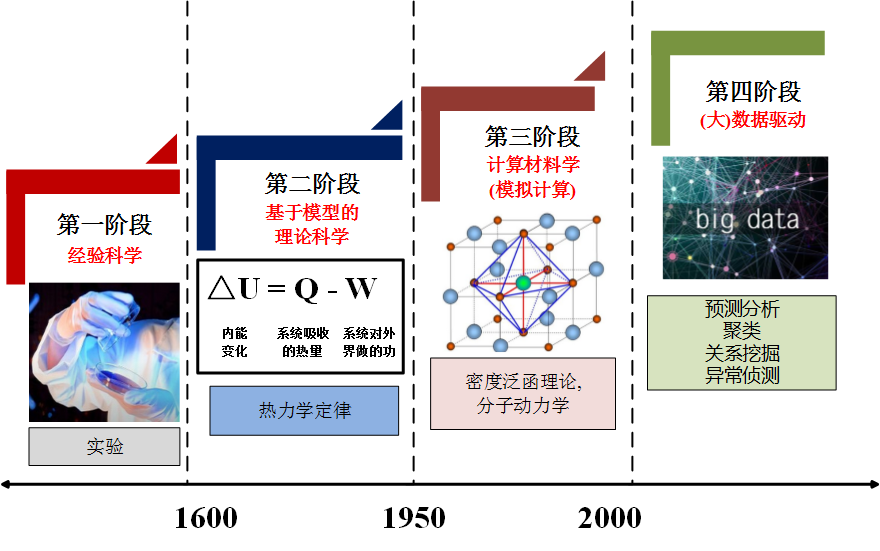
\includegraphics[width=4.05in]{Figures/Four_Model.png}
%\caption{\tiny \textrm{Pseudopotential for metallic sodium, based on the empty core model and screened by the Thomas-Fermi dielectric function.}}%(与文献\cite{EPJB33-47_2003}图1对比)
\label{Four_Model}
\end{figure}
}

\frame
{
	\frametitle{材料模拟的基本思想和方法}
\begin{figure}[h!]
\vspace*{-0.20in}
\centering
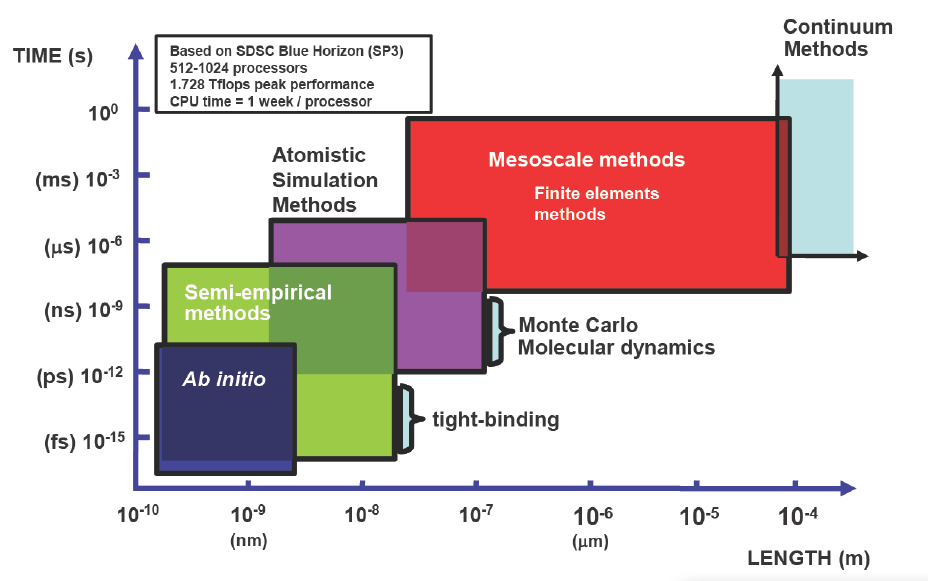
\includegraphics[height=2.20in,width=3.45in]{Figures/Multi-Scale-6.png}
\vskip 0.05pt
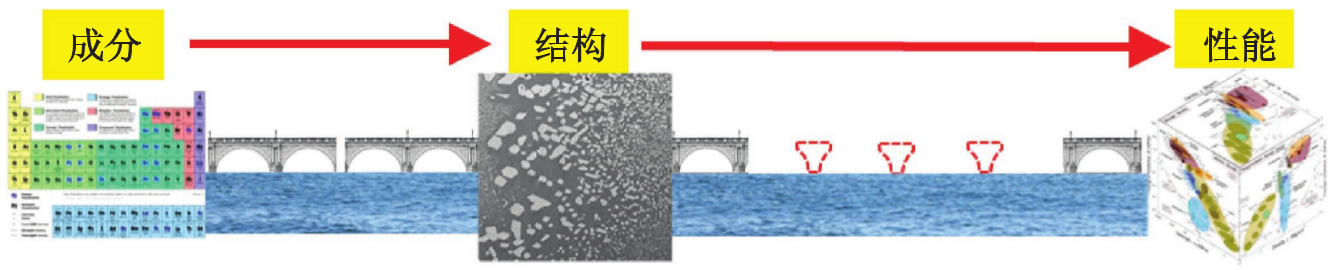
\includegraphics[height=0.80in,width=4.05in]{Figures/MGE-2.png}
%\caption{\tiny \textrm{Pseudopotential for metallic sodium, based on the empty core model and screened by the Thomas-Fermi dielectric function.}}%(与文献\cite{EPJB33-47_2003}图1对比)
\label{Multi-Scale}
\end{figure}
}

\section{量子力学基础}
\frame
{
	\frametitle{量子力学的奠基人}
\begin{figure}[h!]
\centering
%\vspace{-25.5pt}
%\hspace*{-15.5pt}
%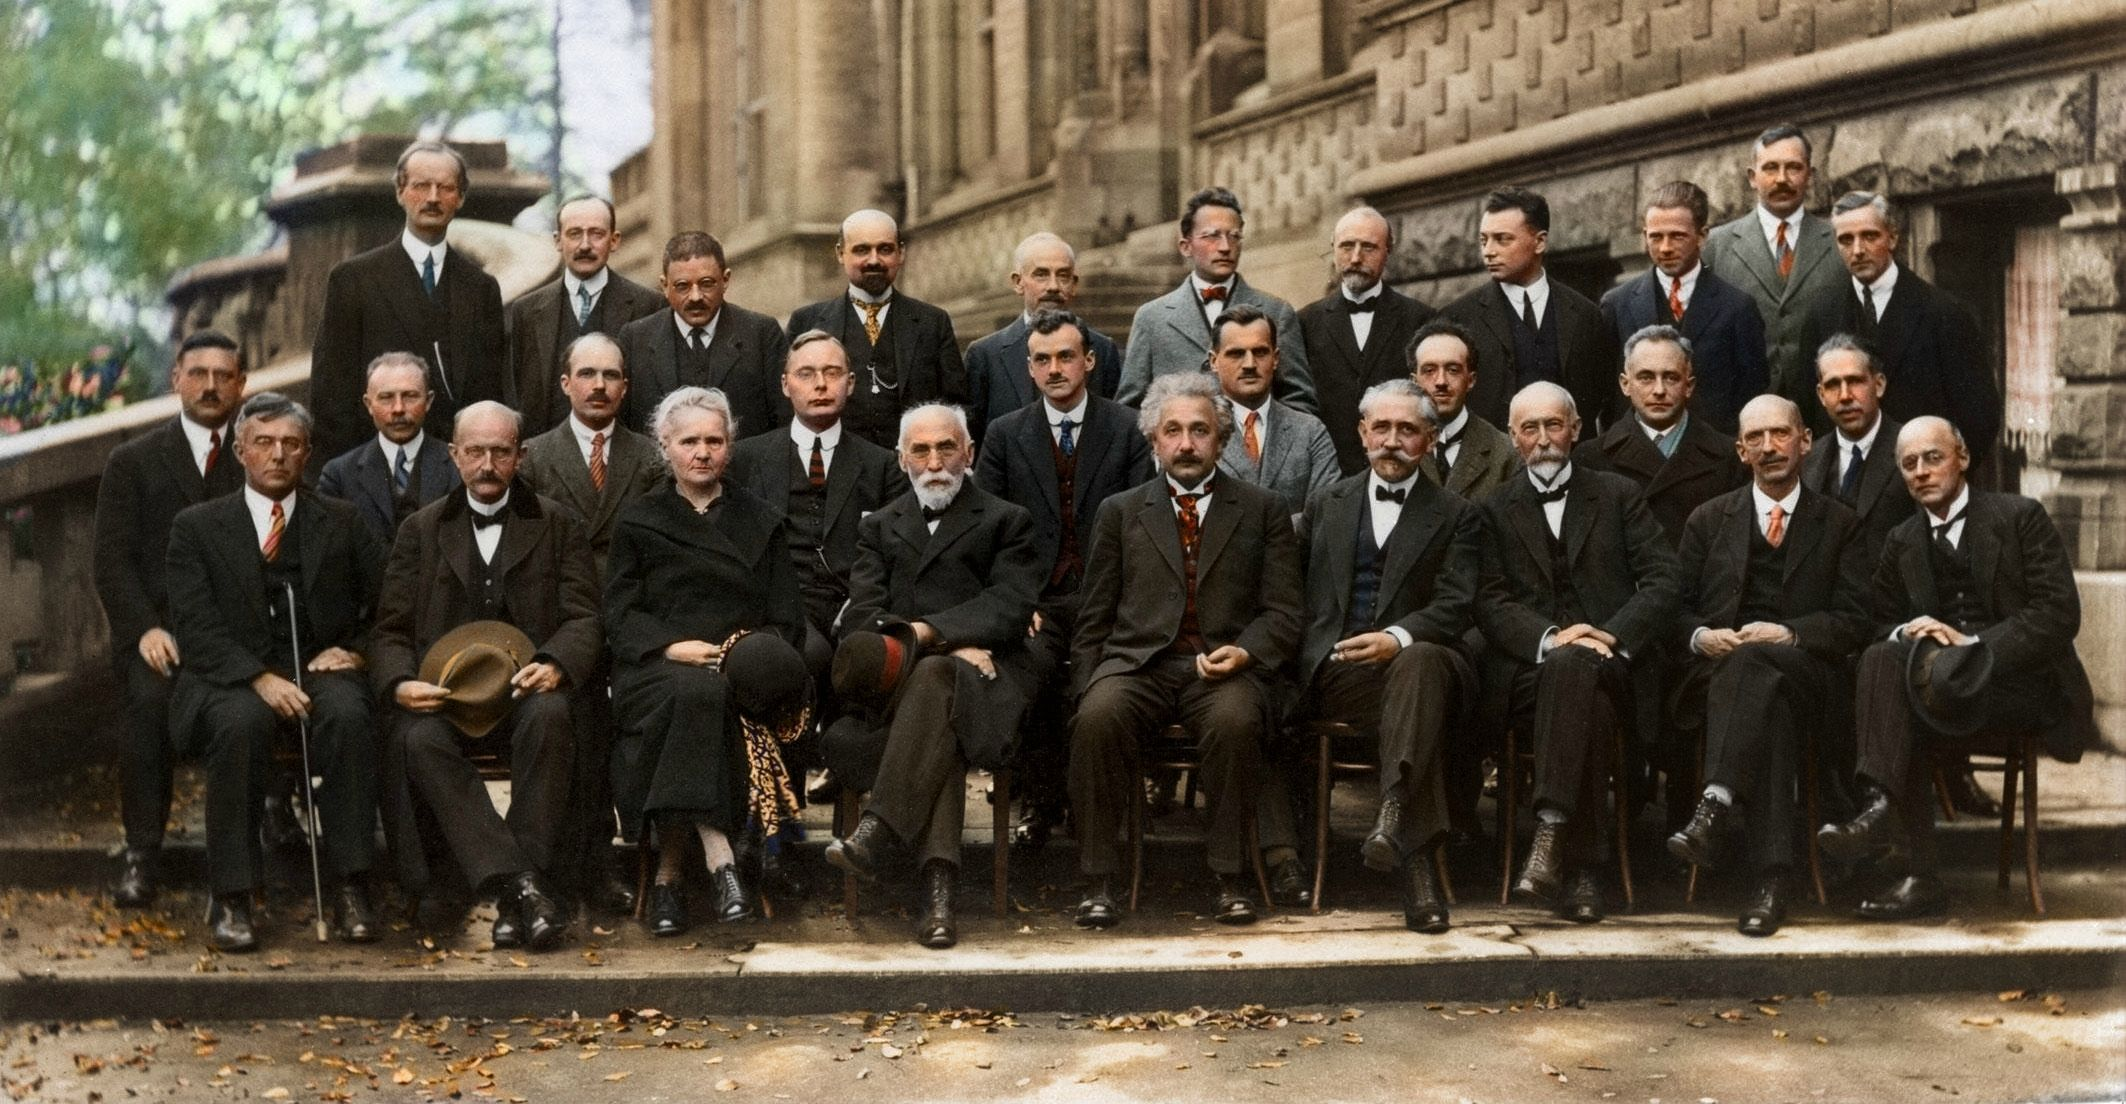
\includegraphics[height=0.57\textwidth,width=1.1\textwidth,viewport=0 0 2150 1050,clip]{Figures/Solvay_Conference-5-fine.jpg}
\vspace{-14.5pt}
\hspace*{-15.5pt}
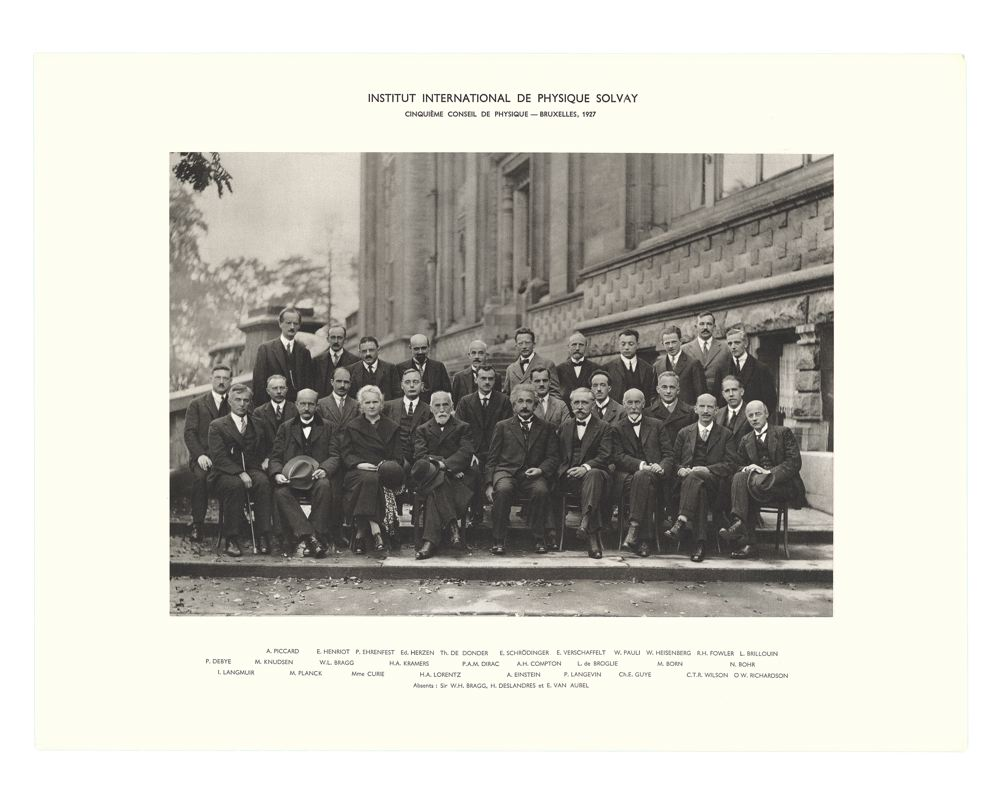
\includegraphics[height=0.55\textwidth,width=0.70\textwidth,viewport=150 105 850 710,clip]{Figures/Solvay_Conference-5.jpg}
\caption{\fontsize{6.5pt}{6.2pt}\selectfont{\textrm{The Fifth Solvay International Conference, Brussels, Belgium, Oct. 1927}}}
\label{Solvay Conference-5-fine}
\end{figure}
\vspace{-11.5pt}
\fontsize{4.1pt}{3.9pt}\selectfont{\textrm{\textcolor{blue}{前排左起}:~I.Langmuir(\textcolor{blue}{朗缪尔}) M.Planck(\textcolor{blue}{普朗克}) Marie Curie(\textcolor{blue}{居里夫人}) H.Lorentz(\textcolor{blue}{洛仑兹}) A.Einstein(\textcolor{blue}{爱因斯坦}) P.Langevin(\textcolor{blue}{朗之万}) Ch.E.Guye(\textcolor{blue}{古伊}) C.T.R.Wilson(\textcolor{blue}{威尔逊}) O.W.Richardson(\textcolor{blue}{理查森})\\
\textcolor{blue}{中排左起}:~P.Debye(\textcolor{blue}{德拜}) M.Knudsen(\textcolor{blue}{克努森}) W.L.Bragg(\textcolor{blue}{布拉格}) H.A.Kramers(\textcolor{blue}{克莱默}) P.A.M.Dirac(\textcolor{blue}{狄拉克}) A.H.Compton(\textcolor{blue}{康普顿}) L.de Broglie(\textcolor{blue}{德布罗意}) M.Born(\textcolor{blue}{玻恩}) N.Bohr(\textcolor{blue}{玻尔})\\
\textcolor{blue}{后排左起}:~A.Piccard(\textcolor{blue}{皮卡尔德}) E.Henriot(\textcolor{blue}{亨利厄特}) P.Ehrenfest(\textcolor{blue}{埃伦费斯特}) Ed.Herzen(\textcolor{blue}{赫尔岑}) Th.de Donder(\textcolor{blue}{德唐德}) E.Schr\"odinger(\textcolor{blue}{薛定谔}) E.Verschaffelt(\textcolor{blue}{费尔夏费尔特}) W.Pauli(\textcolor{blue}{泡利}) W.Heisenberg(\textcolor{blue}{海森堡}) R.H.Fowler(\textcolor{blue}{富勒}) L.Brillouin(\textcolor{blue}{布里渊})}}
}
%------------------------------------------------------------------------Reference----------------------------------------------------------------------------------------------
\frame
{
	\frametitle{黑体辐射与能量量子化}
	\textrm{1900}年,为了解释黑体辐射\textrm{(black-body radiation)}的能量密度与辐射频率的关系,\textrm{M.~Planck}引入\textcolor{red}{能量量子化}的假设,利用统计物理推导出与实验符合得非常好的黑体辐射\textrm{Planck~}公式:~
	\begin{displaymath}
		\rho_{\nu}\mathrm{d}{\nu}=\dfrac{8{\pi}h{\nu}^3}{C^3}\bigg(\dfrac1{\mathrm{e}^{h\nu/kT}-1}\bigg)\mathrm{d}\nu
	\end{displaymath}
\begin{figure}[h!]
\centering
\vspace{-10.5pt}
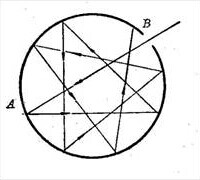
\includegraphics[height=1.45in,width=1.45in,viewport=0 0 136 136,clip]{Figures/Black_box.jpg}
\hskip 1pt
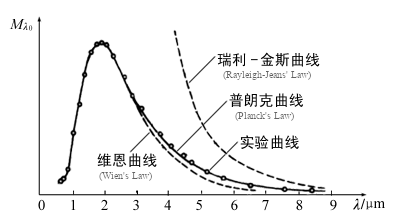
\includegraphics[height=1.32in,width=2.25in,viewport=0 0 390 215,clip]{Figures/Black_box_curve.png}
\caption{\textrm{The black-body radiation and the curve}}
\label{Black_box}
\end{figure}
}

\frame
{
	\frametitle{量子力学基本假设(\textcolor{red}{公理体系})}
	\begin{itemize}
		\item 全同粒子假设\\
			\textcolor{blue}{全同粒子组成的体系中,两个全同粒子相互调换不改变体系的状态}\\ 
			全同粒子是指\textcolor{red}{内禀性质完全相同的一类微观粒子}:\\例如,所有的电子是全同粒子 
		\item 波函数假设\\
			\textcolor{blue}{微观体系的运动状态可由波函数$\Psi$完全描述,波函数包含体系的所有性质}\\
			波函数$\Psi$一般要求满足\textcolor{red}{连续}、\textcolor{red}{有限}和\textcolor{red}{单值}三个条件
		\item 态叠加原理\\
			如果$\Psi_1$是体系的一个本征态,对应的本征值为$A_1$,$\Psi_2$也是体系的一个本征态,对应的本征值为$A_2$,则\textcolor{blue}{$$\Psi=C_1\Psi_1+C_2\Psi_2$$}\textcolor{red}{也是体系一个可能的存在状态}
	\end{itemize}
}

\frame
{
	\frametitle{Schr\"odinger's cat}
\begin{figure}[h!]
\centering
\vspace{-10.5pt}
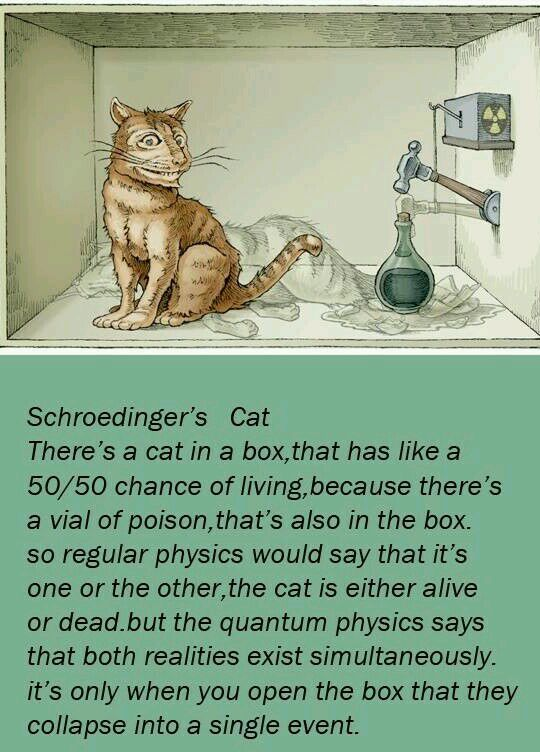
\includegraphics[height=0.70\textwidth,width=0.7\textwidth,viewport=0 0 760 750,clip]{Figures/Schrodinger-cat.jpg}
%\caption{\textrm{ABINIT}的Si.in}
\label{Schrodinger-cat}
\end{figure}
}

\frame
{
	\frametitle{量子力学基本假设(续)}
	\begin{itemize}
		\item 力学量算符假设\\
			\textcolor{blue}{经典力学中的物理量对应到量子力学中,要用线性\textrm{Hermite~}算符表示}(\textcolor{red}{\textrm{Hermite~}算符的本征函数构成完备空间})\\
			如动量算符 
			$$\hat{\mathbf{p}}=-\mathrm{i}\hbar\nabla$$
			位置算符$$\hat{\mathbf r}=r$$
			力学量算符之间有确定的对易关系(量子条件)
			$$[\hat{\mathbf F},\hat{\mathbf G}]=\hat{\mathbf F}\hat{\mathbf G}-\hat{\mathbf G}\hat{\mathbf F}$$ 
			
		\item 微观体系的运动状态\textcolor{blue}{波函数随时间变化的规律}:\\\textcolor{red}{遵从\textrm{Schr\"odinger}方程}
			$$\mathrm{i}\hbar\dfrac{\mathrm{d}}{\mathrm{d}t}|\Psi\rangle=\hat{\mathbf H}|\Psi\rangle$$
	\end{itemize}
}

%\frame
%{
%	\frametitle{\rm{Paul Dirac's Commandments}}
%	\textrm{\textcolor{purple}{The fundamental laws necessary for the mathematical treatment of a large part of physics and the whole of chemistry are thus completely known, and the difficulty lies only in the fact that application of these laws leads to equations that are too complex to be solved.}}
%}

\section{\rm{Hartree-Fock~}方法}
\frame
{
	\frametitle{\textrm{Born-Oppenheimer~}近似}
	\begin{itemize}
		\item 由于原子核的质量要比电子大很多(一般要大3-4个数量级),在同样的相互作用下,原子核的运动比电子也慢得多
		\item 电子在每一时刻仿佛运动在静止原子核构成的势场中,而原子核运动时则感受不到电子的具体位置,感受到的是运动电子的平均作用力
		\item 可近似将原子核坐标与电子坐标变量分离,使得求解整个体系的波函数的复杂过程分解为求解电子波函数和求解原子核波函数两个相对简单的过程\\
			电子运动方程$$\hat{\mathbf H}_{\mathrm e}(\vec r,\vec{\mathbf R})\Psi(\vec r,\vec{\mathbf R})=E_{\mathrm e}(\vec{\mathbf R})\Psi(\vec r,\vec{\mathbf R})$$
			原子核运动方程$$[\hat{\mathbf T}_{\mathrm{nul}}+E_{\mathrm e}(\vec{\mathbf R})]\chi(\vec{\mathbf R})=E\chi(\vec{\mathbf R})$$
	\end{itemize}
}

\frame
{
	\frametitle{独立粒子近似}
	\textrm{n-}粒子体系中的每个粒子的运动,完全忽略粒子间的瞬时相互作用,认为第$i$个粒子在其余$\mathrm{n}-1$个粒子组成的平均势场中运动
	$$\Psi(\vec r_1,\vec r_2,\vec r_3,\cdots,\vec r_n)=\psi_1(\vec r_1)\psi_2(\vec r_2)\psi_3(\vec r_3)\cdots\psi_n(\vec r_n)$$
	$$\hat{\mathbf H}=\sum_{i=1}^N-\dfrac{1}{2}\nabla_i^2+\sum_{i=1}^NV_i(\vec r_i)+\sum_{i,j(j\neq i)}\dfrac{e^2}{|\vec r_i-\vec r_j|}$$
	粒子$i$的\textrm{Hartree}算符
	$$\hat{\mathbf h}_i=-\dfrac{1}{2}\nabla_i^2+V_i(r_i)+\sum_{j(j\neq i)}^N\dfrac{e^2}{|\vec r_i-\vec r_j|}$$
	因此每个粒子的运动方程为:
	$$\hat{\mathbf h}_i\psi_i(\vec r)=\bigg[-\dfrac{1}{2}\nabla_i^2+V_i(r_i)+\sum_{j(j\neq i)}^N\dfrac{e^2}{|\vec r_i-\vec r_j|}\bigg]\psi_i(\vec r)=\varepsilon\psi_i(\vec r)$$ 
}

\frame
{
	\frametitle{\textrm{Slater~}行列式}
	简单乘积的独立粒子波函数不满足全同粒子置换对称性要求,不能正确表示电子不可辨认的物理属性
	
	\textrm{Slater}建议用行列式形式表示具有反对称性的波函数
	\begin{displaymath}
		\hspace*{-10pt}\Psi(\vec r_1,\vec r_2,\vec r_3,\cdots,\vec r_n)=\dfrac1{\sqrt{n!}}
		\left|\begin{array}{ccccc}
			\psi_1(\vec r_1)&\psi_2(\vec r_1)&\psi_3(\vec r_1)&\cdots&\psi_n(\vec r_1)\\
			\psi_1(\vec r_2)&\psi_2(\vec r_2)&\psi_3(\vec r_2)&\cdots&\psi_n(\vec r_2)\\
			\psi_1(\vec r_3)&\psi_2(\vec r_3)&\psi_3(\vec r_3)&\cdots&\psi_n(\vec r_3)\\
			&&&\cdots&\\
			\psi_1(\vec r_n)&\psi_2(\vec r_n)&\psi_3(\vec r_n)&\cdots&\psi_n(\vec r_n)
		\end{array}\right|
	\end{displaymath}
	粒子$i$的\textrm{Fock}算符
	$$\hat{\mathbf F}_i=-\dfrac{1}{2}\nabla_i^2+V_i(r_i)+\hat{\mathbf J}_i-\hat{\mathbf K}_i$$
	$$\hat{\mathbf J}_i(\vec r_i)=\int\dfrac{\psi_j^{\ast}(\vec r_j)|e^2|\psi_j(\vec r_j)}{|\vec r_i-\vec r_j|}\mathrm{d}\vec r_j$$
	$$\hat{\mathbf K}_i(\vec r_i)\psi_i(\vec r_i)=\psi_j(\vec r_i)\int\dfrac{\psi_j(\vec r_j)|e^2|\psi_i(\vec r_j)}{|\vec r_i-\vec r_j|}\mathrm{d}\vec r_j$$

}

\frame
{
	\frametitle{\textrm{Hartree-Fock-Roothan~}方法}
	实际求解非相对论的\textrm{Schr\"odinger}方程时,
	$$\hat{\mathbf F}_i\psi_i(\vec r_i)=\varepsilon_i\psi_i(\vec r_i)$$
	将波函数$\psi_i(\vec r_i)$用一套选定的基函数$\phi_j(\vec r)$展开
	$$\psi_i(\vec r)=\sum_{j=1}^Nc_{ij}\phi_j(\vec r)$$
	通过变分原理
	$$\bar E=\dfrac{\langle\Psi|\hat{\mathbf H}|\Psi\rangle}{\langle\Psi|\Psi\rangle}\geqslant E_0$$
	改变展开系数$c_{ij}$直到体系的能量最小,确定展开系数

	重复上述流程直至\textrm{Fock}算符$\hat{\mathbf F}$、波函数$\psi(\vec r)$和能量$\varepsilon$自洽,这就是\textrm{Hartree-Fock-Roothan}方法
}

%\frame
%{
%	\frametitle{\textrm{RHF~}与\textrm{UHF}} 
%	\begin{itemize}
%		\item \textrm{RHF}:\\
%			针对闭壳层(\textrm{closed shell})体系,占据轨道的电子成对出现,自旋相反,可用一个\textrm{Slater}行列式表示\\
%	%		每对自旋相反的电子有相同的轨道波函数\\
%			对于闭壳层体系,\textrm{Hartree-Fock}方法求解的能量本征值符合\textrm{Koopmans}定理
%			$$E_{ion}^1=-\varepsilon_{\mathrm{HOMO}}$$
%		\item \textrm{UHF}:\\
%			针对开壳层(\textrm{open shell})体系,占据轨道有未成对电子,需要用\textrm{Slater}行列式的线性组合表示\\
%			最低能态用一个\textrm{Slater}行列式,但不同自旋的轨道分别处理
%		$$E_{\mathrm{UHF}}\leqslant E_{\mathrm{RHF}}$$
%			由于\textrm{UHF}包含更多的变分函数,可以处理一些近解离极限的分子体系
%	\end{itemize}
%}
%
\frame
{
	\frametitle{\textrm{Slater~}的$\chi_{\alpha}$方法}
	由于\textrm{Hartree-Fock~}的交换势计算复杂,\textrm{Slater~}建议用电子密度的加权平均来简化交换势的求解
	\begin{displaymath}
		V_{\mathrm x}=-\frac{\sum\limits_i\sum\limits_jn_in_j\int\varphi_i^{\ast}(\vec r)\varphi_i(\vec r{}^{\prime})(2/|\vec r-\vec r{}^{\prime}|)\varphi_j^{\ast}(\vec r{}^{\prime})\varphi_j(\vec r)\mathrm{d}\vec r}{\sum\limits_kn_k\varphi_k^{\ast}(\vec r)\varphi_k(\vec r)}
	\end{displaymath}
	自由电子气在动量空间用\textrm{Hartree-Fock}方法表示
	\begin{displaymath}
		V_{\mathrm x}(k)=-8\left( \frac3{8\pi}\rho \right)^{1/3}F(\eta)
	\end{displaymath}
	这里$\eta=k/k_{\mathrm F}$,并有
	\begin{displaymath}
		F(\eta)=\frac12+\frac{1-\eta^2}{4\eta}\ln\left|\frac{1+\eta}{1-\eta}\right|
	\end{displaymath}
	$F(\eta)$在$\eta=1(k=k_{\mathrm F})$出现奇点(对应于自由电子气\textrm{Fermi~}面上电子密度为0)。
}
	
%\frame
%{
%	\frametitle{\textrm{Slater~}的$\chi_{\alpha}$方法}
%	\textrm{Slater~}建议,对占据态($k\leqslant k_{\mathrm F}$)的电子作加权平均,可有
%	\begin{displaymath}
%		F(\eta)=\frac{\int_0^1\eta^2F(\eta)\mathrm{d}\eta}{\int_0^1\eta^2\mathrm{d}\eta}=\frac34
%	\end{displaymath}
%	因此,对于均匀电子气,交换势
%	\begin{displaymath}
%		V_{\mathrm x}=-6\left( \frac3{8\pi}\rho \right)^{1/3}
%	\end{displaymath}
%	\textrm{Slater~}指出,对于局域电子密度$\rho(\vec r)$体系,可有\textrm{Slater~}交换势
%	\begin{displaymath}
%		V_{\mathrm xs}(\vec r)=-6\left( \frac3{8\pi}\rho(\vec r) \right)^{1/3}
%	\end{displaymath}
%	在此基础上,\textrm{Slater~}建议对上述交换势引入可调参数$\alpha$,有交换势
%	\begin{displaymath}
%		V_{\chi_{\alpha}}(\vec r)=\alpha V_{\mathrm xs}(\vec r)
%	\end{displaymath}
%}
%
\frame
{
	\frametitle{交换与相关}
	\begin{itemize}
		\item \textrm{Fock}算符中的交换算符$\hat{\mathrm K}_i(\vec r_i)$是由\textrm{Slater}行列式引入的,属于量子效应
	\end{itemize}
%	\vspace*{-5pt}
	\begin{displaymath}
%		\hspace*{-2pt}
		\text{电子间瞬时相互作用(\textcolor{red}{关联})}
		\left\{
			\begin{aligned}
				&\text{\textcolor{blue}{电子交换}:同自旋电子的关联作用}\\
				&\text{\textcolor{blue}{电子相关}}
			\end{aligned}
			\right.
	\end{displaymath}
\begin{figure}[h!]
\centering
\vspace{-10.5pt}
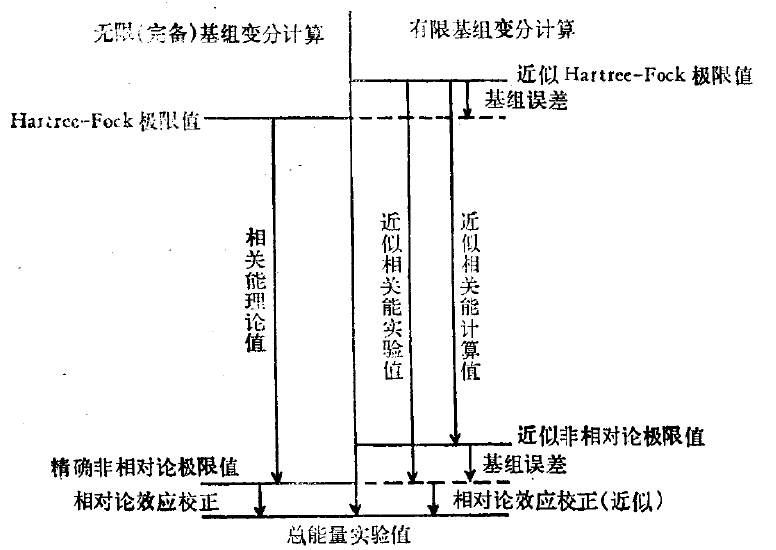
\includegraphics[height=0.42\textwidth,width=0.6\textwidth,viewport=0 0 760 550,clip]{Figures/Post-HF.png}
%\caption{\textrm{ABINIT}的Si.in}
\label{Post-HF}
\end{figure}
}

%\frame
%{
%	\frametitle{\textrm{Post-HF}}
%	\textrm{Hartree-Fock}方法精确定义了交换作用,完全没考虑电子相关作用
%	\begin{itemize}
%		\item \textrm{CI (Configuration Interaction)}
%	$$\Psi=\sum_{I=0}C_I\Phi_I=C_0\Phi_0+C_1\Phi_1+C_2\Phi_2+\cdots$$
%		\item \textrm{CC (Couple Cluste)}\\
%			\begin{displaymath}
%				\Psi=\mathrm{e}^{\hat{\mathbf T}}\Phi_0=\mathrm{e}^{(\hat{\mathbf T_1}+\hat{\mathbf T_2}+\hat{\mathbf T_3}+\cdots)}\Phi_0
%			\end{displaymath}
%		\item \textrm{MP}微扰方法
%			\begin{displaymath}
%				\begin{aligned}
%					&\hat{\mathbf H}=\hat{\mathbf H}^{(0)}+\hat{\mathbf V} \\
%					&\hat{\mathbf H}^{(0)}=\sum_i\hat{\mathbf F}_i \qquad \Phi^{(0)}=\Psi_{\mathrm{HF}}\\ 
%					&\hat{\mathbf V}=\sum_{j>i}^{occ}\dfrac{e^2}{r_{ij}}-\sum_{ij}^{occ}\big(\hat{\mathbf J}_{ij}-\dfrac12\hat{\mathbf K}_{ij}\big)
%				\end{aligned}
%			\end{displaymath}
%	\end{itemize}
%}
%
\section{密度泛函理论}       %Bookmark
\subsection{\rm{Thomas-Fermi~}模型}       %Bookmark
\frame
{
	\frametitle{\textrm{Thomas-Fermi}模型} 
	1927年,\textrm{Thomas}和\textrm{Fermi}基于均匀电子气模型上建立\textrm{Thomas-Fermi}模型,\textcolor{blue}{体系能量可用}\textcolor{red}{电子密度}\textcolor{blue}{表示}:
	\begin{itemize}
		\item 动能表达式
			$$T_{\mathrm{TF}}[\rho(\vec r)]=\dfrac3{10}(3\pi^2)^{\frac23}\int\rho^{\frac53}(\vec r)\mathrm{d}\vec r$$
		\item 外势$V_{ext}(\vec r)$下电子体系的能量泛函表达式为
			\begin{displaymath}
				\begin{aligned}
					E_{\mathrm{TF}}[\rho(\vec r)]=&\dfrac3{10}(3\pi^2)^{\frac23}\int\rho^{\frac53}(\vec r)\mathrm{d}\vec r\\
					&+\int\rho(\vec r)V_{ext}(\vec r)\mathrm{d}\vec r+\dfrac12\int\int\dfrac{\rho(\vec r_1)\rho(\vec r_2)}{|\vec r_2-\vec r_1|}\mathrm{d}\vec r_1\mathrm{d}\vec r_2
				\end{aligned}
			\end{displaymath}
		\item \textrm{Thomas-Fermi}模型完全没有考虑电子的交换-相关作用
	\end{itemize}
}

\frame
{
	\frametitle{\textrm{Thomas-Fermi-Dirac}模型} 
	1930年,\textrm{Dirac}将\textrm{Thomas-Fermi}模型修正,用局域密度近似考虑电子交换作用
			\begin{displaymath}
				\begin{aligned}
					E_{\mathrm{TFD}}[\rho(\vec r)]=&\dfrac3{10}(3\pi^2)^{\frac23}\int\rho^{\frac53}(\vec r)\mathrm{d}\vec r+\int\rho(\vec r)V_{ext}(\vec r)\mathrm{d}\vec r\\
					&+\dfrac12\int\int\dfrac{\rho(\vec r_1)\rho(\vec r_2)}{|\vec r_2-\vec r_1|}\mathrm{d}\vec r_1\mathrm{d}\vec r_2-\dfrac34\bigg(\dfrac3{\pi}\bigg)^{\frac13}\int\rho^{\frac43}(\vec r)\mathrm{d}\vec r
				\end{aligned}
			\end{displaymath}
			\begin{itemize}
				\item 在总电子数守恒约束条件
					$$\int\rho(\vec r)\mathrm{d}\vec r=N$$
					下,能量泛函$E_{\mathrm{TFD}}[\rho(\vec r)]$对密度$\rho(\vec r)$的变分极小获得体系的基态密度和基态能量
			\end{itemize}
}

\frame
{
	\frametitle{\textrm{Thomas-Fermi}模型}
	\begin{itemize}
		\item \textrm{Thomas-Fermi}模型用电子密度代替波函数描述问题是极大的简化,但模型过于粗糙:\\
%			\begin{enumerate}
%				\item 以均匀电子气的密度得到动能的表达式
%				\item 完全忽略电子间的交换-相关作用
%			\end{enumerate}
			不能正确描述相互作用电子体系的基本特征,如原子的壳层结构
		\item \textrm{Thomas-Fermi}模型虽不够精确,但可以通过引入修正项校正:
			\textrm{Dirac}交换泛函 $$E_X[\rho(\vec r)]=-\dfrac34\bigg(\dfrac3{\pi}\bigg)^{\frac13}\int\rho^{\frac43}(\vec r)\mathrm{d}\vec r$$
			\textrm{Wigner}相关泛函 $$E_C[\rho(\vec r)]=-0.056\int\dfrac{\rho^{\frac43}(\vec r)}{0.079+\rho^{\frac13}(\vec r)}\mathrm{d}\vec r$$
	\end{itemize}
	\textrm{Thomas-Fermi}模型为密度泛函理论\textrm{(DFT)}提供了重要的启示
}

\subsection{密度泛函理论}       %Bookmark
\frame                               %
{
\frametitle{密度泛函理论(\textrm{DFT})} %Slide Page Title
%   \secname
与传统的量子力学方法不同,密度泛函理论的基本变量是体系的基态电子密度。%通过体系的电子密度而非波函数确定体系的基态能量。
\begin{itemize}%[+-| alert@+>]
	\item 密度泛函理论的基石:\textrm{Hohenberg-Kohn}定理\upcite{PR136-B864_1964}
\vskip 5pt
\begin{itemize}%[+-| alert@+>]
   \setlength{\itemsep}{8pt}
 \item $E[\rho]=F_{\mathrm{HK}}[\rho]+\displaystyle\int\rho(\vec{r})v(\vec{r})\textrm{d}\vec{r}$ \\
\vskip 5pt 其中$F_{\mathrm{HK}}[\rho]=\underset{\Psi\to\rho}{\mathrm{Min}}\langle\Psi[\rho]|\hat{T}+\hat{W}|\Psi[\rho]\rangle$
是普适的泛函表达式。%,指明多电子体系的基态性质与基态密度间存在一一对应关系
     \textrm{\small{第一定理表明多电子体系的性质完全由体系的基态密度决定}}
   \item 如果$\tilde\Psi\neq\Psi$,
     $E[\tilde\rho]\geqslant E[\rho_0]$\\
     \textrm{\small{第二定理指出基态总能量泛函在体系基态电子密度处取极小值}}
   \end{itemize}
%\textrm{\small{第二定理指出基态总能量泛函在体系基态电子密度处取极小值}}
\vskip 8pt
 \item 密度泛函理论的优越性:用密度($\rho$)代替波函数($\Psi$)描述体系
\vskip 5pt
 \item 密度泛函理论的困难:能量密度泛函的精确形式未知
   \end{itemize}
}

\frame                               %
{
\frametitle{密度泛函理论(\textrm{DFT})}
\textrm{Kohn-Sham}方程\upcite{PR140-A1133_1965}:无相互作用体系+交换-相关能的贡献
$$(T_S+V_{e\!f\!f})|\varphi_i\rangle=\varepsilon_i|\varphi_i\rangle,\quad i=1,\cdots,N,\cdots$$
其中$T_S=-\dfrac12\nabla^2$~~是无相互作用体系的动能\\
$V_{e\!f\!f}(\vec r)=V_{ext}(\vec r)+\displaystyle\int w(\vec r,\vec r\,')\rho(\vec r\,')\mathrm{d}\vec r\,'+V_{\mathrm{XC}}[\rho]$
\vskip 5pt
$V_{ext}(\vec r)$是电子体系与外部的电荷或磁场相互作用\\
$V_{\mathrm{XC}}[\rho]=\dfrac{\delta E_{\mathrm{XC}}}{\delta\rho(\vec r)}$称为交换-相关势
\vskip 10pt
\textrm{Kohn-Sham}方程是形式上的单粒子方程
\vskip 6pt
\textrm{Kohn-Sham}方程的实质:\\\textcolor{red}{将动能泛函的主要部分分离出来,剩余部分放在交换-相关能中}
}

\frame
{
\frametitle{交换-相关能与交换-相关势}
实际考虑交换-相关能时,会将交换-相关能表示为交换能和相关能之和:
\begin{displaymath}
	E_{\mathrm{XC}}[\rho]=E_{\mathrm{X}}[\rho]+E_{\mathrm{C}}[\rho]=\int\varepsilon_{\mathrm{X}}[\rho]\rho(\vec{r}) \textrm{d}^3\vec{r}+\int\varepsilon_{\mathrm{C}}[\rho]\rho(\vec{r}) \textrm{d}^3\vec{r}
\end{displaymath}
$\varepsilon_{\mathrm{X}}[\rho]$和$\varepsilon_{\mathrm{C}}[\rho]$可理解为单电子的交换能和相关能
\vskip 20pt
交换-相关势通过交换-相关能计算得到:~
		\begin{displaymath}
			V_{\mathrm{XC}}^{\sigma}[\rho_{\alpha},\rho_{\beta}]=\dfrac{\delta E_{\mathrm{XC}}[\rho_{\alpha},\rho_{\beta}]}{\delta\rho_{\sigma}}=\dfrac{\delta\{E_{\mathrm{X}}[\rho_{\alpha},\rho_{\beta}]+E_{\mathrm{C}}[\rho_{\alpha},\rho_{\beta}]\}}{\delta\rho_{\sigma}}
		\end{displaymath}
		\textcolor{red}{注意}:~由于$E_{\mathrm{XC}}[\rho_{\sigma}]$对$\rho_{\sigma}$是非线性的\\
		\textcolor{blue}{$V_{\mathrm{XC}}=V_{\mathrm{X}}+V_{\mathrm{C}}$和$\varepsilon_{\mathrm{XC}}=\varepsilon_{\mathrm{X}}+\varepsilon_{\mathrm{C}}$不同,不要混淆这两个量}
}
%  \beamertemplateshadingbackground{blue!10}{yellow!10}

\frame                               %
{
\frametitle{交换-相关能密度泛函}
\textcolor{blue}{密度泛函理论的核心问题}:\\
\textrm{Kohn-Sham}方程用于实际计算,必须知道$E_{XC}[\rho]$或者$V_{XC}[\rho]$与$\rho(\vec r)$的泛函关系
\vskip 15pt
\begin{minipage}[b]{0.59\textwidth}
 \hspace*{-15pt}
 {\fontsize{7.5pt}{6.0pt}\selectfont\begin{itemize}%[+-| alert@+>]
	 \setlength{\itemsep}{10pt}
 \item \textrm{LDA}:泛函只与密度分布的局域值有关
 \item \textrm{GGA}:泛函依赖:局域密度及其梯度
 \item $meta$-\textrm{GGA}:泛函依赖的变量还有动能密度
 \item 杂化(\textrm{hybrid})泛函:泛函与占据轨道有关
 \item 其他的交换-相关能泛函
 \item<1-> 完全非局域泛函:理想泛函,不现实
 \end{itemize}}
\end{minipage}
\hfill
\begin{minipage}[b]{0.39\textwidth}
\hspace*{-10pt}
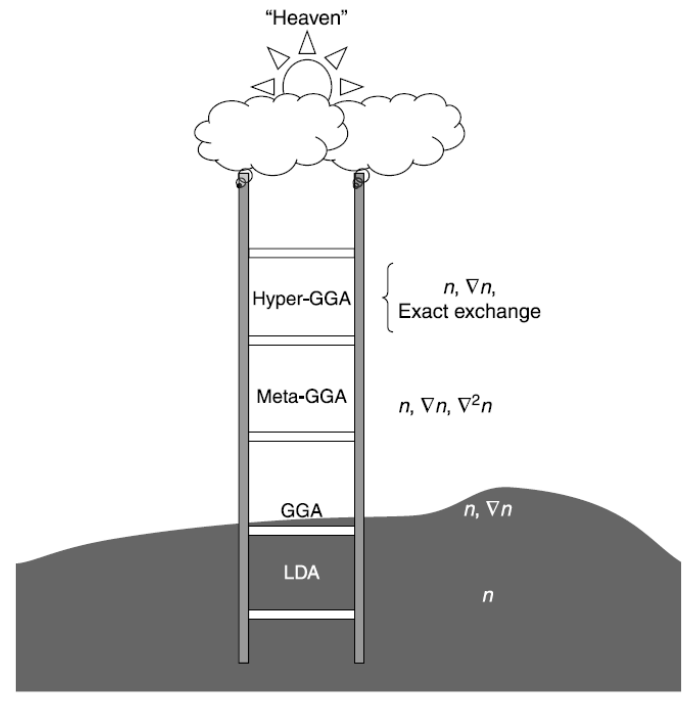
\includegraphics[height=1.7in,width=3.18in,viewport=10 5 1380 700,clip]{Figures/Jacobi-ladder.png}\\
\centering{\textcolor{red}{\textrm{\tiny Jacob's ladder}}}
\end{minipage}
% \begin{itemize}%[+-| alert@+>]
%\item 交换-相关能密度泛函
}

\frame%[allowframebreaks]
{
	\frametitle{\rm{LDA}泛函}
	\begin{itemize}
		\item 交换能部分
	\begin{displaymath}
		\begin{aligned}
			\varepsilon_{\mathrm{X}}[\rho,\zeta]=&2^{-1/3}C_{\mathrm{X}}^{\sigma}g(\zeta)\rho^{1/3}(\vec r)\\
			E_{\mathrm{X}}[\rho,\zeta]=&\int\varepsilon_{\mathrm{X}}[\rho,\zeta]\rho(\vec r)\mathrm{d}\vec r\\
		\end{aligned}
	\end{displaymath}
	{\fontsize{7.5pt}{6.0pt}\selectfont{这里:~$C_{\mathrm{X}}^{\sigma}=\dfrac32\bigg(\dfrac3{4\pi}\bigg)^{1/3}$\\
		$g(\zeta)=\dfrac12\bigg[(1+\zeta)^{4/3}+(1-\zeta)^{4/3}\bigg]$\\
		$\zeta(\vec r)=\dfrac{[\rho_{\alpha}(\vec r)-\rho_{\beta}(\vec r)]}{[\rho_{\alpha}(\vec r)+\rho_{\beta}(\vec r)]}$}}
	\end{itemize}
}

\frame%[allowframebreaks]
{
	\frametitle{\rm{LDA}泛函}
	\begin{itemize}
		\item 相关能部分
			\begin{displaymath}
				\hspace*{-30pt}	\varepsilon_{\mathrm{C}}^{\mathrm{LDA}}(r_s,\zeta)=\varepsilon_{\mathrm{C}}(r_s,0)+a_{\mathrm{c}}(r_s)\dfrac{f(\zeta)}{f^{\prime\prime}(\zeta)}(1-\zeta^4)+[\varepsilon_{\mathrm{c}}(r_s,1)-\varepsilon_{\mathrm{c}}(r_s,0)]f(\zeta)\zeta^4
			\end{displaymath}
			{\fontsize{7.5pt}{6.0pt}\selectfont{这里:~$r_s=\bigg[\dfrac3{4\pi}(\rho_{\alpha}+\rho_{\beta})^{-1}\bigg]^{1/3}$~$f(\zeta)=[(1+\zeta)^{4/3}+(1-\zeta)^{4/3}-2]/(2^{4/3}-2)$\\
			$\varepsilon_{\mathrm{C}(r_s,0)}$、$\varepsilon_{\mathrm{C}(r_s,1)}$、$a_{\mathrm{C}(r_s)}$由经验公式
			\begin{displaymath}
				\begin{aligned}
					&G(r_s,A,\alpha_1,\beta_1,\beta_2+\beta_3+\beta_4)\\
					=&-2A(1+\alpha_1r_s)\ln\bigg[1+\dfrac1{2A(\beta_1r_s^{1/2}+\beta_2r_s+\beta_2r_s^{3/2}+\beta_1r_s^2)}\bigg]
				\end{aligned}
			\end{displaymath}
		计算。其中$A$、$\alpha_1$、$\beta_1$、$\beta_2$、$\beta_3$、$\beta_4$是参数,通过拟合实验结果确定}}
		\begin{displaymath}
			E_{\mathrm{C}}[\rho]=\int\rho(\vec r)\varepsilon_{\mathrm{C}}(\vec r)\mathrm{d}\vec r
		\end{displaymath}
	\end{itemize}
}

\subsection{\rm{LDA}与精确交换-相关泛函}
\frame                               %
{
	\frametitle{近似能量泛函$E_{\mathrm{XC}}[\rho]$的主要问题}
\vskip 20pt
\begin{enumerate}%[+-| alert@+>]
   \setlength{\itemsep}{10pt}
 \item  密度是整体变量:~电子自相互作用抵消不净\\%\quad\textrm{(LDA+U)}方法的校正%(\textrm{LDA+U})
	 用\textrm{DFT}计算电子数很少的体系,一般都会有较大的误差
 \item  电子相关:~简并和近简并基态的表示不合理\\
	 基态电子密度用不同的简并轨道计算时,体系能量应保持不变,但现有的近似能量泛函不具有这个性质
 \item  渐近行为:~处理弱相互作用体系的误差大\\
	 如\textrm{Van der Waals}相互作用和现有近似能量泛函本身的计算误差在同一量级
 \end{enumerate}
}

\frame
{
	\frametitle{\textrm{L(S)DA}方法的不足}
	\begin{itemize}
		\item 一般对只含$s$、$p$价电子体系,基于\textrm{DFT(L(S)DA/GGA)\,}的结构、能带计算都能给出令人满意的结果
		\item 但是对价电子包含$d$和$f$局域电子体系,特别是过渡金属氧化物或氮化物(\textcolor{orange}{如\textrm{Mott}\,绝缘体}),在“金属/绝缘体”的定性判断上,\textrm{L(S)DA/GGA}\,计算结果常常出错
	\end{itemize}
\begin{figure}[h!]
\centering
\vspace*{-0.35in}
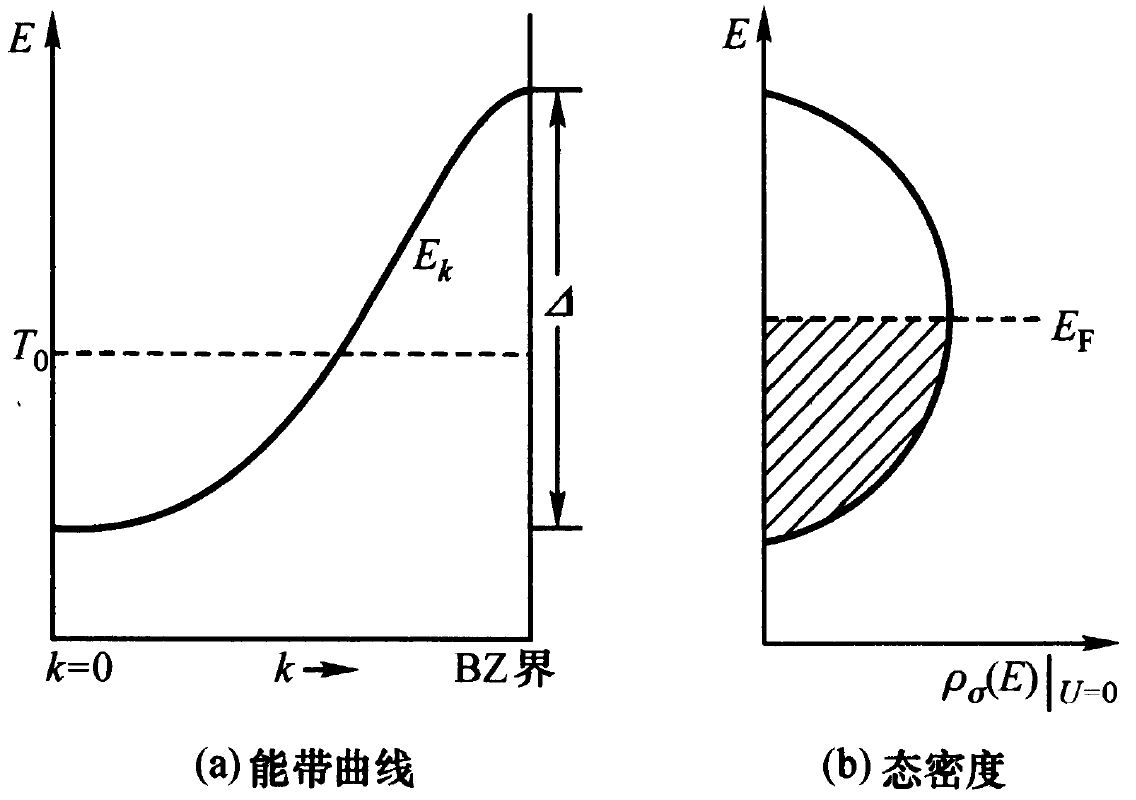
\includegraphics[height=2.05in,width=3.2in,viewport=0 0 1200 880,clip]{Figures/LDA_U-3.png}
\caption{\tiny \textrm{The schematic band structure (a) and DOS (b) of systems including localized electrons calculated based on LDA.}}%(与文献\cite{EPJB33-47_2003}图1对比)
\label{LDA_U-3}
\end{figure}
}

\frame
{
	\frametitle{\textrm{L(S)DA}方法的不足}
\begin{itemize}
\setlength{\itemsep}{12pt}
	\item 精确密度泛函具有当电子数在整数值前后改变的时候,体系能量的改变是不连续的属性,单电子能量的不连续对能带的带隙有很大贡献
	 \item\textrm{LD(S)A~}近似中体系能量是电子数的连续函数,不具备体系能量随电子数变化不连续的特征。\textrm{LDA/GGA~}方法在描述含有$d$/$f$电子的过渡金属和稀土元素化合物体系时常常失效。
	\item \textrm{LDA}/\textrm{GGA~}得到的体系总能量和实验结果符合较好,但轨道能量(即$\varepsilon_i=\partial E/\partial n_i$),不符合\textrm{Koopmans~}定理,与实验或者严格计算得到的轨道能量差别很大%一个典型的例子就是对H原子的计算结果,LDA计算的轨道能级为$-$0.27\,a.u.(实验结果为$-$0.5\,a.u.),总能量($-$0.488\,a.u.)则非常接近$-$0.5\,a.u.\upcite{PRB37-9919_1988}。
%	\item \textrm{Anisimov~}提出通过对\textrm{LDA~}势加入轨道校正克服不足(称为\textrm{LDA+$U$}方法)\upcite{PRB44-943_1991,PRB48-16929_1993}%LDA+U方法与Andersen掺杂模型\upcite{PR124-41_1961}思想类似,
\end{itemize}
}

\frame
{
	\frametitle{精确交换-相关泛函的特征}
	\textrm{Perdew}指出\upcite{PRL49-1691_1982},尽管交换-相关泛函的精确形式不知,但总能量泛函对电子数的依赖$E(N)$应该具有折线形式
\begin{figure}[h!]
\centering
\vspace*{-0.4in}
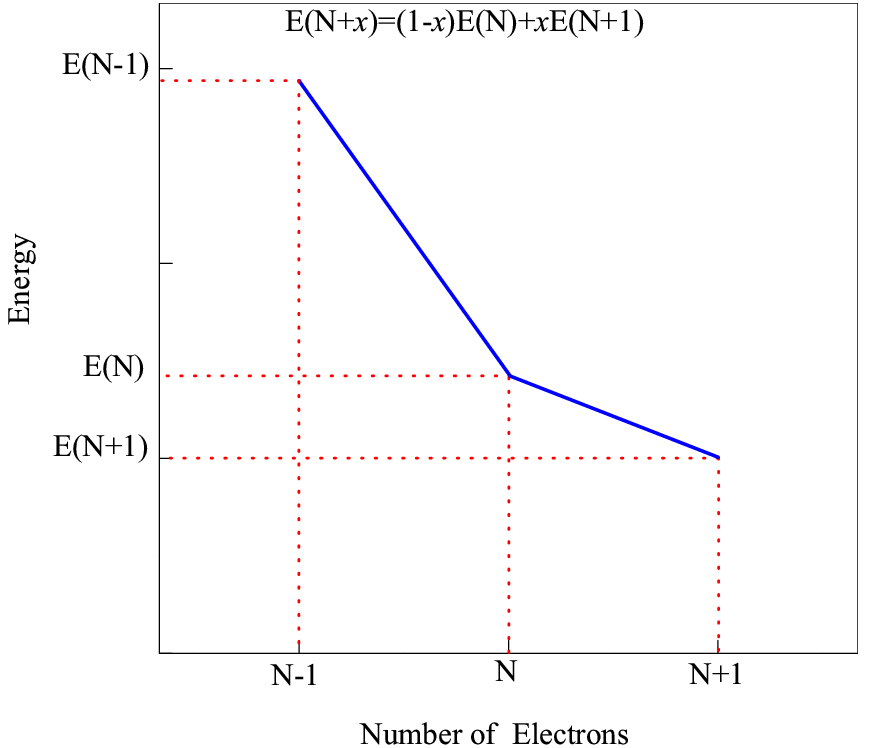
\includegraphics[height=2.4in,width=2.8in,viewport=0 0 1000 880,clip]{Figures/exact-DFT.png}
\caption{\tiny \textrm{The dependence of the total energy on the number of electron is a series of straight-line segments.}}%(与文献\cite{EPJB33-47_2003}图1对比)
\label{exact-DFT}
\end{figure}
}

\frame
{
	\frametitle{\textrm{L(S)DA}与精确交换-相关泛函}
	\begin{itemize}
		\item $E(N)$\textcolor{blue}{曲线本身连续}
	\begin{displaymath}
		\dfrac{\partial E}{\partial N}=\left\{
		\begin{aligned}
			E(M)-E(M-1)\qquad M-1<N<M\\
			E(M+1)-E(M)\qquad M<N<M+1 
		\end{aligned}\right.
	\end{displaymath}
		\item 导数$\partial E/\partial N$\textcolor{red}{在跨越整数电子时不连续}

	类似地,精确的单电子势$V(\vec r)=\dfrac{\delta E}{\delta n(\vec r)}$\\
	\textcolor{blue}{在电子数出现整数变化时同样存在不连续的跳跃}
		\item \textrm{L(S)DA}近似下,能量$E$对电子数$N$曲线及其导数\textcolor{red}{\underline{都是连续的}}
	
			\vspace{10pt}
	\textcolor{blue}{\textrm{L(S)DA}近似对\textrm{Mott}绝缘体计算的失效}:\\
	\textcolor{red}{单电子势函数不满足电子数整数变化时跳跃的不连续要求}
	\end{itemize}
}

\subsection{交换-相关泛函的改进}
\frame%[allowframebreaks]
{
	\frametitle{\rm{GGA}泛函}
	\begin{itemize}
		\item 交换能泛函:
			\begin{itemize}
				\item \textrm{PW91}
					\begin{displaymath}
						\begin{aligned}
							E_{\mathrm{X}}^{\mathrm{PW91}}[\rho_{\alpha},\rho_{\beta}]=&\dfrac12(E_{\mathrm{X}}^{\mathrm{PW91}}[2\rho_{\alpha}]+E_{\mathrm{X}}^{\mathrm{PW91}}[2\rho_{\beta}])\\
							E_{\mathrm{X}}^{\mathrm{PW91}}[\rho]=&-\dfrac34\bigg(\dfrac3\pi\bigg)^{1/3}\int\rho^{4/3}(\vec r)F(x)\mathrm{d}\vec r
						\end{aligned}
					\end{displaymath}
					\hspace*{-30 pt}{\fontsize{4.5pt}{4.0pt}\selectfont{这里:~$F(x)=\dfrac{1+0.19645(hx)\sinh^{-1}(7.7956hx)+(hx)^2\{0.2743-0.1508\mathrm{exp}[-100(hx)^2]\}}{1+0.19645(hx)\sinh^{-1}(7.7956hx)+0.004(hx)^4}$}\\
					$h=(24\pi^2)^{-1/3}$,~~~$x=|\nabla\rho|\rho^{-4/3}$}
				\item \textrm{PBE}
			\begin{displaymath}
				E_{\mathrm{X}}^{\mathrm{PBE}}[\rho,x]=E_{\mathrm{X}}^{\mathrm{LDA}}[\rho,x]-C_{\mathrm{X}}\int a\bigg(1-\dfrac1{bx^2}\bigg)\rho^{4/3}(\vec r)\mathrm{d}\vec r
			\end{displaymath}
			{\fontsize{4.5pt}{4.0pt}\selectfont{其中:~$C_{\mathrm{X}}=\dfrac34\bigg(\dfrac3\pi\bigg)^{1/3}$\\$a=0.804$,~~~$b=0.273$~是非经验参数}}
			\end{itemize}
	\end{itemize}
}

\frame%[allowframebreaks]
{
	\frametitle{\rm{GGA}泛函}
	\begin{itemize}
		\item 相关能泛函:
			\begin{itemize}
				\item \textrm{PW91}
					\begin{displaymath}
						\begin{aligned}
							E_{\mathrm{C}}^{\mathrm{PW91}}[\rho_{\alpha},\rho_{\beta}]=&\int\mathrm{d}\vec r\rho(\vec r)[\varepsilon_{\mathrm{C}}^{\mathrm{LSDA}}(r_s,\zeta)]+H(t,r_s,zeta)\\
							H=&H_0+H_1
						\end{aligned}
					\end{displaymath}
					{\fontsize{4.5pt}{4.0pt}\selectfont{这里:~
						\begin{displaymath}
							\begin{aligned}
								H_0=&f^3(\zeta)\dfrac{\beta^2}{2\alpha}\ln\bigg(1+\dfrac{2\alpha}{\beta}\dfrac{t^2+At^4}{1+At^2+A^2t^4}\bigg)\\
								A=&\dfrac{2\alpha}{\beta}\dfrac1{\mathrm{exp[-2\alpha\varepsilon_{\mathrm{C}}^{\mathrm{LDA}}(r_s,\zeta)}/f^3(\zeta)\beta^2]-1}\\
							t=&\dfrac{|\nabla\rho|}{2f(\zeta)k_s\rho}~~~f(\zeta)=\dfrac12\bigg[(1+\zeta)^{2/3}+(1-\zeta)^{2/3}\bigg]\\
							k_s=&[4(3\pi^{-1}\rho)^{1/3}]^{1/2}
							\end{aligned}
						\end{displaymath}
						参数 $\alpha=0.09$,~~~$\beta=\nu C_{\mathrm{C}}(0)$\\
						$\nu=(16/\pi)(3\pi^2)^{1/3}$,~~~$C_{\mathrm{C}}(0)=0.004235$
				}}
			\end{itemize}
	\end{itemize}
}

\frame%[allowframebreaks]
{
	\frametitle{\rm{meta-GGA}泛函}
	\begin{itemize}
		\item 交换能泛函
			\begin{itemize}
				\item \textrm{TPSS}
					\begin{displaymath}
						\begin{aligned}
							E_{\mathrm{X}}^{\mathrm{TPSS}}[\rho]=\int\mathrm{d}\vec r\rho(\vec r)\varepsilon_{\mathrm{X}}^{\mathrm{LSDA}}(\vec r)F_{\mathrm{X}}^{\mathrm{LSDA}}(p,z)\\
							F_{\mathrm{X}}^{\mathrm{TPSS}}=1+\kappa-\dfrac{\kappa}{1+x/\kappa}
						\end{aligned}
					\end{displaymath}
{\fontsize{4.5pt}{4.0pt}\selectfont{这里:~
	$\rho(\vec r)=\rho_{\alpha}(\vec r)+\rho_{\beta}({\vec r})$,~~~$\varepsilon_{\mathrm{X}}^{\mathrm{LSDA}}(\vec r)=-\dfrac3{4\pi}[3\pi^2\rho(\vec r)]^{1/3}$
\\
\begin{displaymath}
	\begin{aligned}
		x=&\left\{\bigg[\dfrac{10}{81}+\dfrac{cz^2}{(1+z^2)^2}\bigg]p+\dfrac{146}{2025}\bar{q}_b^2-\dfrac{73}{405}\bar{q}_b\bigg[\dfrac12\bigg(\dfrac35z\bigg)^2+\dfrac12p^2\bigg]^{1/2}\right.\\
		&+\left.\dfrac1{\kappa}\bigg(\dfrac{10}{81}\bigg)^2p^2\dfrac{20e^{1/2}}{81}\bigg(\dfrac35z\bigg)^2+e\mu p^3\right\}(1+e^{1/2}p)^{-2}\\
		p=&\dfrac{|\nabla\rho(\vec r)|^2}{4(3\pi^2)^{2/3}\rho^{8/3}(\vec r)}, ~~~ \bar{q}_b=\dfrac{(9/20)(\alpha-1)}{[1+b\alpha(\alpha-1)]^{1/2}}+2p/3
	\end{aligned}
\end{displaymath}
$z=\tau_w/\tau$,~~~$\tau_w=\dfrac{|\nabla\rho(\vec r)|^2}{8\rho(\vec r)}$,~~~$\tau=\sum\limits_{\sigma}\tau_{\sigma}$\\
$\alpha=(\tau-\tau_w)/\tau_{\mathrm{unif}}=(5p/3)(z^{-1}-1)$,~~~$\tau_{\mathrm{tiff}}=\dfrac3{10}(3\pi^2)^{2/3}[\rho(\vec r)]^{5/3}$
}}
			\end{itemize}
	\end{itemize}
}


\frame%[allowframebreaks]
{
	\frametitle{\rm{meta-GGA}泛函}
	\begin{itemize}
		\item 相关能泛函
			\begin{itemize}
				\item {\textrm{TPSS}}
					\begin{displaymath}
						E_{\mathrm{C}}^{\mathrm{TPSS}}[\rho_{\alpha,\rho_{\beta}}]=\int\mathrm{d}\vec r\rho(\vec r)\varepsilon_{\mathrm{C}}^{\mathrm{TPSS0}}[1+\mathrm{d}\varepsilon_{\mathrm{C}}^{\mathrm{TPSS0}}(\tau_w/\tau)^3]
					\end{displaymath}
{\fontsize{4.5pt}{4.0pt}\selectfont{这里:~
	\begin{displaymath}
		\begin{aligned}
			\varepsilon_{\mathrm{C}}^{\mathrm{TPSS0}}=&\varepsilon_{\mathrm{C}}^{\mathrm{PBE}}(\rho_{\alpha},\rho_{\beta},\nabla\rho_{\alpha},\nabla\rho_{\beta})[1+C(\zeta,\xi)(\tau_w/\tau)^2]\\
			&-\bigg[1+C(\zeta,\xi)(\tau_w/\tau)^2\sum\limits_{\sigma}\dfrac{\rho_{\sigma}(\vec r)}{\rho(\vec r)}\bar{\varepsilon}_{\mathrm{C}}\bigg]\\
			\bar{\varepsilon}_{\mathrm{C}}=&\max[\varepsilon_{\mathrm{C}}^{\mathrm{PBE}}(\rho_{\alpha},0,\nabla\rho_{\alpha},0),\varepsilon_{\mathrm{C}}^{\mathrm{PBE}}(\rho_{\alpha},\rho_{\beta},\nabla\rho_{\alpha},\nabla\rho_{\beta})]\\
			C(\zeta,\xi)=&\dfrac{C(\zeta,0)}{\{1+\xi^2[(1+\zeta)^{-4/3}+(1-\zeta)^{-4/3}]/2\}^4}
		\end{aligned}
	\end{displaymath}
	$\xi=\dfrac{|\nabla\zeta|}{2[3\pi^2\rho(\vec r)]^{1/3}}$, ~~~$C(\zeta,0)=0.53+0.87\zeta^2+0.50\zeta^4+2.26\zeta^6$
}}
			\end{itemize}
	\end{itemize}
	\vskip 5pt
	\textrm{TPSS}泛函的特点:~\\
	\vskip 3pt
	{\fontsize{7.5pt}{6.0pt}\selectfont{不包含依靠实验数据的可调参数,数字系数由精确能量泛函满足的条件确定\\
		\textcolor{blue}{对电子分布较为均匀的晶体体系和电子分布激烈变化的分子体系都有较高的精度} }}
}

\frame
{
	\frametitle{\rm{hybrid}泛函}
	体系\textrm{Hamilton}算符表示为
	\begin{displaymath}
		\hat{H}_{\lambda}=-\dfrac12\sum_i^N\nabla^2+\sum_i^NV_i(\rho,\lambda)+\dfrac{\lambda}2\sum_i^N\sum_{j(j\neq i)}^N\dfrac1{r_{ij}}
	\end{displaymath}
	\begin{displaymath}
		\mbox{\textcolor{blue}{$\lambda$表征电子间相互作用程度}}\left\{
		\begin{aligned}
			&\lambda=0:~\mbox{无相互作用的参考体系}\\
			&\lambda=1:~\mbox{存在相互租用的真实体系}
		\end{aligned}
		\right.
	\end{displaymath}
	交换-相关能表示为
	\begin{displaymath}
		\begin{aligned}
			E_{\mathrm{XC}}^{\lambda}=&\dfrac12\int\mathrm{d}\vec r_1\rho_1^{\lambda}(\vec r_1)\int\dfrac{h_{\mathrm{XC}}^{\lambda}(\vec r_1,\vec r_2)}{\vec r_1-\vec r_2}\mathrm{d}\vec r_2\\
			E_{\mathrm{XC}}=&\int E_{\mathrm{XC}}^{\lambda}\mathrm{d}\lambda
		\end{aligned}
	\end{displaymath}
	{\fontsize{4.5pt}{4.0pt}\selectfont{这里:~$h_{\mathrm{XC}}(\vec r_1,\vec r_2)=\dfrac{2\rho_2(\vec r_1,\vec r_2)}{\rho(\vec r_1)}-\rho_1(\vec r_2)$}}
}

\frame
{
	\frametitle{\rm{hybrid}泛函}
	\begin{itemize}
		\item \textrm{half-to-half}
			\begin{displaymath}
				\begin{aligned}
					E_{\mathrm{XC}}=&\dfrac12(E_{\mathrm{XC}}^0+E_{\mathrm{XC}}^1)=\dfrac12E_{\mathrm{XC}}^{\mathrm{Exact}}+\dfrac12E_{\mathrm{XC}}^1\\
					\approx&\dfrac12E_{\mathrm{XC}}^{\mathrm{HF}}+\dfrac12E_{\mathrm{XC}}^{\mathrm{LSDA}}
				\end{aligned}
			\end{displaymath}
		\item \textrm{B3LYP}
			\begin{displaymath}
			\hspace*{-20pt}	E_{\mathrm{XC}}^{\mathrm{B3LYP}}=(1-a)E_{\mathrm{X}}^{\mathrm{LSDA}}+aE_{\mathrm{X}}^{\mathrm{HF}}+b\Delta E_{\mathrm{X}}^{\mathrm{VB88}}+cE_{\mathrm{C}}^{\mathrm{LYP}}+(1-c)E_{\mathrm{C}}^{\mathrm{LSDA}}
			\end{displaymath}
	\end{itemize}
	\vskip 8pt
	\textcolor{blue}{电子间的交换能和相关能都是离域的,但长程作用方向相反,很大程度上彼此抵消,剩余部分主要是局域的,所以将交换能和相关能合在一起处理,用局域近似可以比较好地描述电子行为}\\
	\vskip 5pt
	\textcolor{red}{采用精确交换能形式,虽然消除了自相互作用的误差,但剩余的相关能主体是离域的,因此局域形式的泛函不再是好的近似,对电子行为的描述效果会变差}
}

\frame
{
%\frametitle{The methods on band structure calculation}
\frametitle{密度泛函计算方法}
%\vskip 10pt
%\textrm{The mainly difference of all these methods below: the basis sets and the construction of the potential}
\vskip 10pt
常用的计算方法
\begin{itemize}%[+-| alert@+>]
%\begin{enumerate}%[+-| alert@+>]
\setlength{\itemsep}{12pt}
%  \item \textrm{Plane wave and the pseudo-potential}
	\item	平面波方法
	\item	正交平面波\textrm{(The orthogonalized plane wave, OPW)}和赝势\textrm{(Pseudo-potential, PP)}方法%\upcite{Singh_Book,PRB41-7892_1990,JPCM6-8245_1994}
	\item	缀加平面波\textrm{(Augmented plane wave, APW)}方法
	\item	\textrm{MT}轨道\textrm{(Muffin-tin orbitals, MTO)}方法
	\item	投影子缀加波\textrm{(Projector Augmented Wave, PAW)}方法%\upcite{PRB50-17953_1994,PRB59-1758_1999}
\end{itemize}
\vskip 5pt 各种方法的\textcolor{red}{主要区别}:~\textcolor{blue}{势函数的处理}与\textcolor{blue}{所选基函数类型}不同
}

\frame
{
%	\frametitle{\textrm{DFT-SCF}}
\begin{figure}[h!]
\vspace*{-0.25in}
\centering
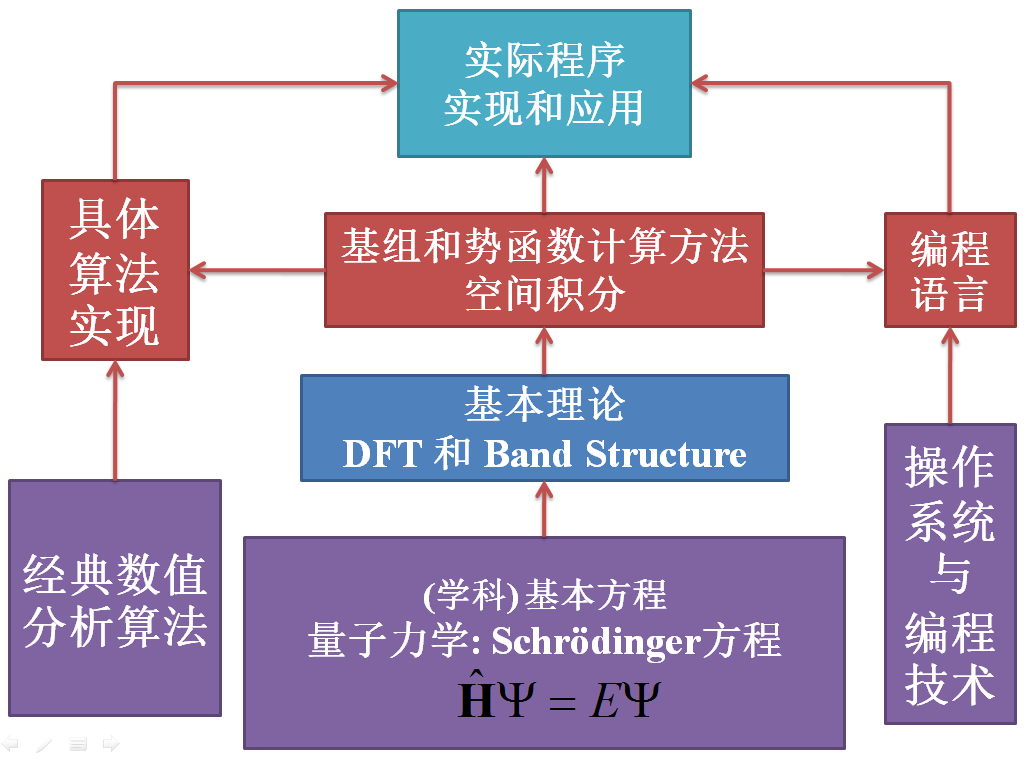
\includegraphics[height=2.80in,width=4.95in,viewport=5 3 1250 780,clip]{Figures/Method_Procedure.png}
%\caption{\tiny \textrm{Pseudopotential for metallic sodium, based on the empty core model and screened by the Thomas-Fermi dielectric function.}}%(与文献\cite{EPJB33-47_2003}图1对比)
\label{Method-Procedure}
\end{figure}
}

\frame
{
	\frametitle{\textrm{DFT-SCF}}
\begin{figure}[h!]
\centering
\vspace*{-0.25in}
\hspace*{-0.80in}
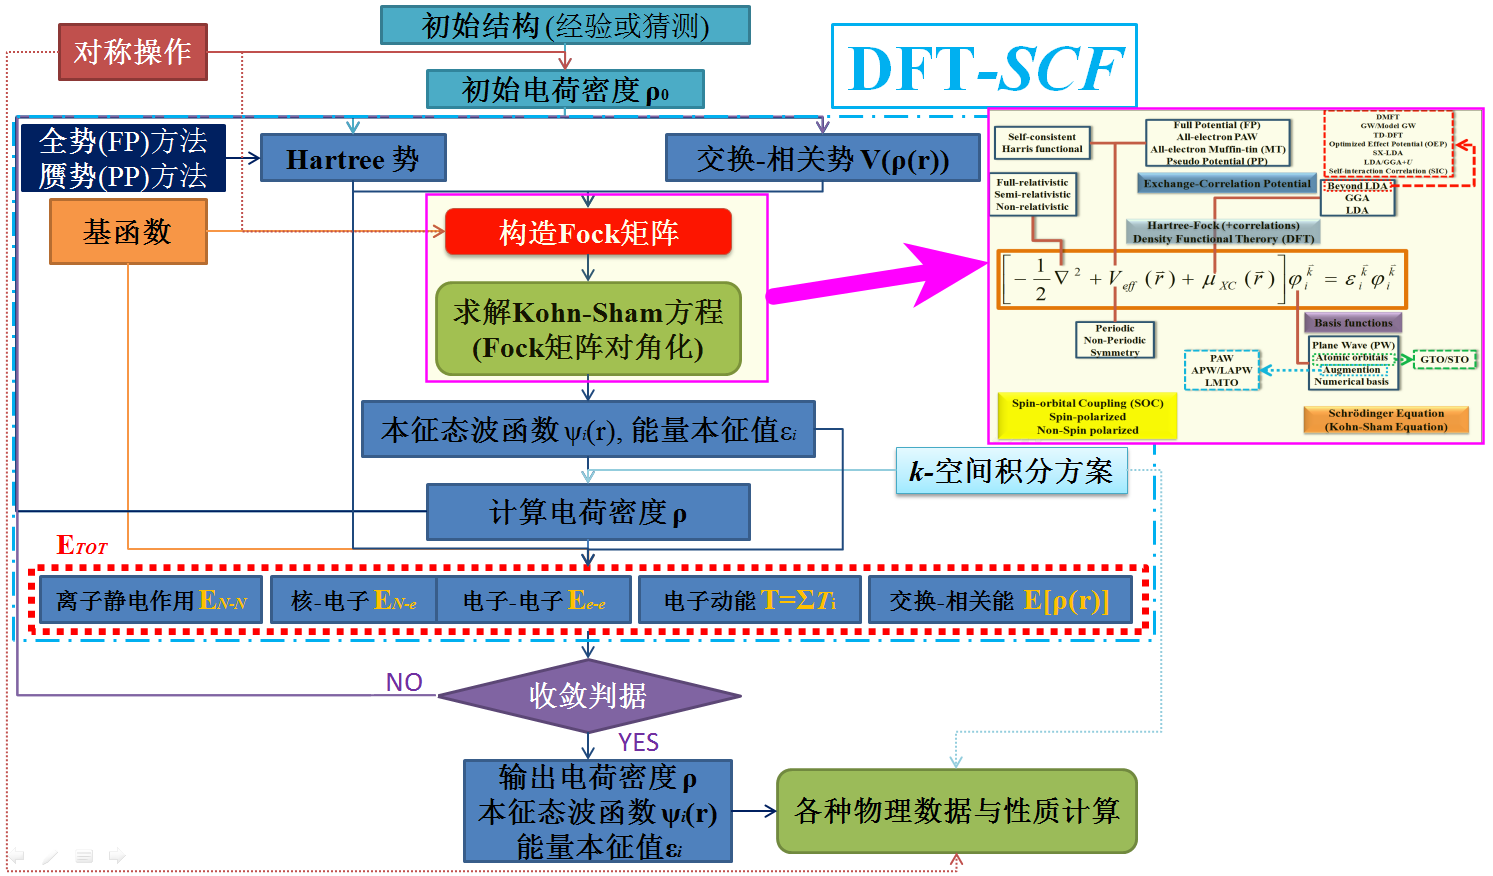
\includegraphics[height=2.80in,width=4.95in,viewport=5 3 1490 870,clip]{Figures/DFT-SCF_2.png}
%\caption{\tiny \textrm{Pseudopotential for metallic sodium, based on the empty core model and screened by the Thomas-Fermi dielectric function.}}%(与文献\cite{EPJB33-47_2003}图1对比)
\label{DFT-SCF-2}
\end{figure}
}

\frame                               %
{
	\frametitle{\textrm{Kohn-Sham}方程}
\begin{figure}[h!]
\centering
\vspace*{-0.21in}
\hspace*{-0.1in}
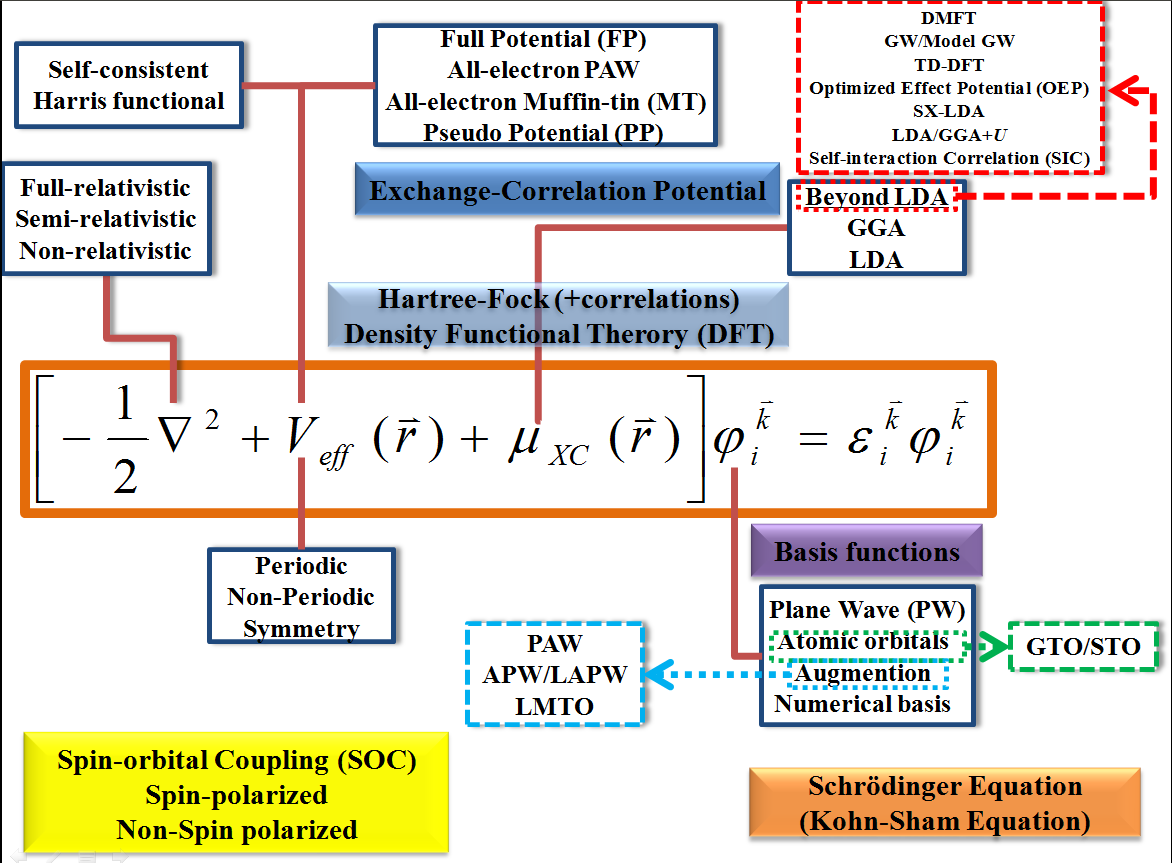
\includegraphics[height=2.7in,width=4.0in,viewport=2 5 1162 880,clip]{Figures/DFT.png}
\caption{\tiny \textrm{The Analysis of Kohn-Sham equation.}}%(与文献\cite{EPJB33-47_2003}图1对比)
\label{DFT}
\end{figure}
}

%------------------------------------------------------------------------Reference----------------------------------------------------------------------------------------------
		\frame[allowframebreaks]
{
\frametitle{主要参考文献}
\begin{thebibliography}{99}
{\tiny
	\bibitem{Xu_Li_Wang}徐光宪、黎乐民、王德民, {\textit{量子化学——基本原理和从头计算法}}\;\textrm{({\textit{上、中}})}\:科学出版社, 北京, 1980
	\bibitem{PR136-B864_1964}\textrm{P. Hohenberg and W. Kohn, \textit{Phys. Rev.} \textbf{136} (1964), B864}
	\bibitem{PR140-A1133_1965}\textrm{W. Kohn and L.J. Sham, \textit{Phys. Rev.} \textbf{140} (1965), A1133}
	\bibitem{PRL49-1691_1982}\textrm{P. Perdew, R. G. Parr, M. Levy and J. L. Balduz, Jr., \textit{Phys. Rev. Lett.} \textbf{49} (1982), 1691}
	\bibitem{Parr_Yang}\textrm{R.G. Parr and W. Yang. \textit{Density-Functional Theory of Atoms and Molecules} (Oxford University Press, New York, U.S.A., 1989)}
}
\end{thebibliography}
\nocite*{}
}
%-----------------------------------------------------------------------------------------------------------------------------------------------------------------------%

%-----------------------------------------------------------Beamer下不建议使用bib,因为涉及分页--------------------------------------------------------------------------%
%\frame[allowframebreaks]
%{
%\frametitle{主要参考文献}
%{\tiny\textrm{
%%\phantomsection\addcontentsline{toc}{section}{Bibliography}	 %直接调用\addcontentsline命令可能导致超链指向不准确,一般需要在之前调用一次\phantomsection命令加以修正	%
%%\phantomsection\addcontentsline{toc}{section}{主要参考文献}	 %直接调用\addcontentsline命令可能导致超链指向不准确,一般需要在之前调用一次\phantomsection命令加以修正	%
%\bibliography{Ref_2020-03-04}%
%\bibliographystyle{../ref/mybib}%
%}}
%\nocite{*}%
%}
%------------------------------------------------------------------------------------------------------------------------------------------------------------------------------%
%\frame[allowframebreaks]
%%{
%\frametitle{主要参考文献}
%{\tiny\textrm{
%%\phantomsection\addcontentsline{toc}{section}{Bibliography}	 %直接调用\addcontentsline命令可能导致超链指向不准确,一般需要在之前调用一次\phantomsection命令加以修正	%
%%\phantomsection\addcontentsline{toc}{section}{主要参考文献}	 %直接调用\addcontentsline命令可能导致超链指向不准确,一般需要在之前调用一次\phantomsection命令加以修正	%
%\bibliography{../ref/Myref}																			%
%\bibliographystyle{../ref/mybib}																		%
%}}
%\nocite{*}																				%
%}
%------------------------------------------------------------------------------------------------------------------------------------------------------------------------------%

%-------------------------------------------------------------------------Thanks------------------------------------------------------------------------------------------------
%\section{致谢}
%\frame
%{
%\frametitle{致$\quad$谢}
%\begin{itemize}
%    \setlength{\itemsep}{20pt}
%  \item 感谢本团队高兴誉、吴泉生、宋红州等各位老师参与的讨论
%  \item 感谢莫所长、宋主任以及软件中心各位老师和同事
%  \item 感谢王崇愚先生的帮助
%\end{itemize}
%}

\logo{}									%不显示logo
\frame
{
\vskip 60 pt
%\hskip 10pt \textcolor{blue}{\Huge 感谢答辩委员会各位老师\,\textrm{!}}\\
\vskip 35 pt
\hskip 60pt \textcolor{blue}{\Huge 谢谢大家\:!}
%\vskip 15 pt
%\hskip 40pt \textcolor{blue}{\Huge \textrm{for your attention\:!}}
}

%\frame
%{
%\begin{figure}[h!]
%\centering
%\animategraphics[autoplay, loop, height=2.1in]{1}{Figures/Prof_Liu-}{06}{11}
%\label{Prof_Liu}
%\end{figure}
%}
%
%-------------------------------------------------------------------------------------------------------------------------------------------------------------------------------

\clearpage
%\end{CJK*}
\end{document}
